\documentclass{beamer}
%\usepackage[T1]{fontenc}
\usepackage[utf8]{inputenc}
%\usepackage{lmodern}  % Use the Latin Modern font family

\usepackage{latexsym,amsmath,xcolor,bm, amssymb, color, tikz, graphicx, amsthm, mathtools}
\usepackage{algorithm}
\usepackage{algorithmic}
\usepackage{hyperref}
\usepackage{float}     
\usepackage{CJKutf8}
\usepackage{multicol}
\usepackage{listings}

\lstset{
  language=C++,
  basicstyle=\ttfamily\small,
  keywordstyle=\color{blue},
  commentstyle=\color{gray},
  stringstyle=\color{orange},
  breaklines=true,
  showstringspaces=false,
  tabsize=2,
  columns=fullflexible,
  keepspaces=true
}

\graphicspath{{../logos/}}

\DeclareMathOperator*{\argmax}{arg\,max}
\DeclareMathOperator*{\argmin}{arg\,min}
\DeclareMathOperator{\sign}{sign}
\DeclareMathOperator{\Tr}{Tr}

\makeatletter
\DeclareRobustCommand\onedot{\futurelet\@let@token\@onedot}
\def\@onedot{\ifx\@let@token.\else.\null\fi\xspace}
\def\eg{\emph{e.g}\onedot} 
\def\Eg{\emph{E.g}\onedot}
\def\ie{\emph{i.e}\onedot} 
\def\Ie{\emph{I.e}\onedot}
\def\cf{\emph{c.f}\onedot} 
\def\Cf{\emph{C.f}\onedot}
\def\etc{\emph{etc}\onedot} 
\def\vs{\emph{vs}\onedot}
\def\wrt{w.r.t\onedot} 
\def\dof{d.o.f\onedot}
\def\etal{\emph{et al}\onedot}
\makeatother


\usetheme{Madrid}
\useinnertheme{circles}


\definecolor{ColorUNLP}{HTML}{8c0011} 
\usecolortheme[named=ColorUNLP]{structure}
%\usecolortheme[named=ColorUNR]{exampleblock}

%\setbeamertemplate{blocks}[rounded][shadow=true]
%\setbeamercolor{block body}{fg=black,bg=white}



%------------------------------------------------------------
%This block of code defines the information to appear in the
%Title page
\title %optional
{Árboles Recargados}

\subtitle{(Consultas en subárboles y en caminos)}

%\subtitle{with applications to persuation and lie production}
% \author % (optional)
% {Author Name}

\author[Sebastián Mestre]{Sebastián Mestre}

\institute[]{Universidad Nacional de Rosario - FCEIA}
\date[TC 2026]{Training Camp 2026}
\titlegraphic{
\includegraphics[clip,height=2cm,keepaspectratio]{logoTC.pdf}}

%End of title page configuration block
%------------------------------------------------------------


%------------------------------------------------------------
% \AtBeginSection inserts an automatic Outline slide at the start of
% each \section{}, highlighting the current section. Change the
% \section names below to your real topic names and these slides
% will update automatically.
\AtBeginSection[]
{
  \begin{frame}
    \frametitle{Outline}
    \tableofcontents[currentsection]
  \end{frame}
}
%------------------------------------------------------------


\begin{document}

%The next statement creates the title page.
\frame{\titlepage}


%------------------------------------------------------------
% Frame de Sponsors, me parece mejor ponerlo al principio
% Antes del índice/contenido

% --- Organizadores y Sponsors ---
\begin{frame}{Gracias Sponsors!}
    \begin{columns}[t]
        \column{0.5\textwidth}
        \centering
        Organiza\\
        \vspace{0.5cm}
        
\includegraphics[width=0.6\textwidth,keepaspectratio]{logo_aapc.png}\\
        \vspace{0.3cm}
        
\includegraphics[width=0.8\textwidth,keepaspectratio]{unlp_informatica.png}
        \column{0.5\textwidth}
        \centering
        Diamond Sponsor\\
        \vspace{0.5cm}
        
\includegraphics[width=0.8\textwidth,keepaspectratio]{GTSlogo.jpeg}
    \end{columns}
\end{frame}


%---------------------------------------------------------
%This block of code is for the table of contents after
%the title page
\begin{frame}
\frametitle{Outline}
\tableofcontents
\end{frame}
%---------------------------------------------------------


\setcounter{tocdepth}{2}

\section{Introducción}
\subsection{Conteo de divisores}

\begin{frame}
  \frametitle{Pregunta}

  \begin{itemize}
    \item Sea \(N\) un número natural: ¿cuántos divisores tiene, en promedio, un número entre \(1\) y \(N\)?
  \end{itemize}

  \vspace{1em}
\end{frame}

\begin{frame}{Conteo doble}
  \[
    D(n) = \{\text{divisores de } n\}
  \]

  \[
    \frac{1}{N} \sum_{n=1}^{N} |D(n)|
  \]

  \[
    \left\{
      (m, n) \in \mathbb{N}^2 \;\middle|\;
      \textcolor{red}{m \mid n}
      \text{ y }
      n \leq N
    \right\}
  \]

  \begin{block}{$m \mid n$}
    \begin{itemize}
      \item ``$m$ divide a $n$''
      \item ``$m$ es divisor de $n$''
      \item ``$n$ es múltiplo de $m$''
      \item $\exists k : n = k m$
    \end{itemize}
  \end{block}
\end{frame}

\begin{frame}
  \centering
  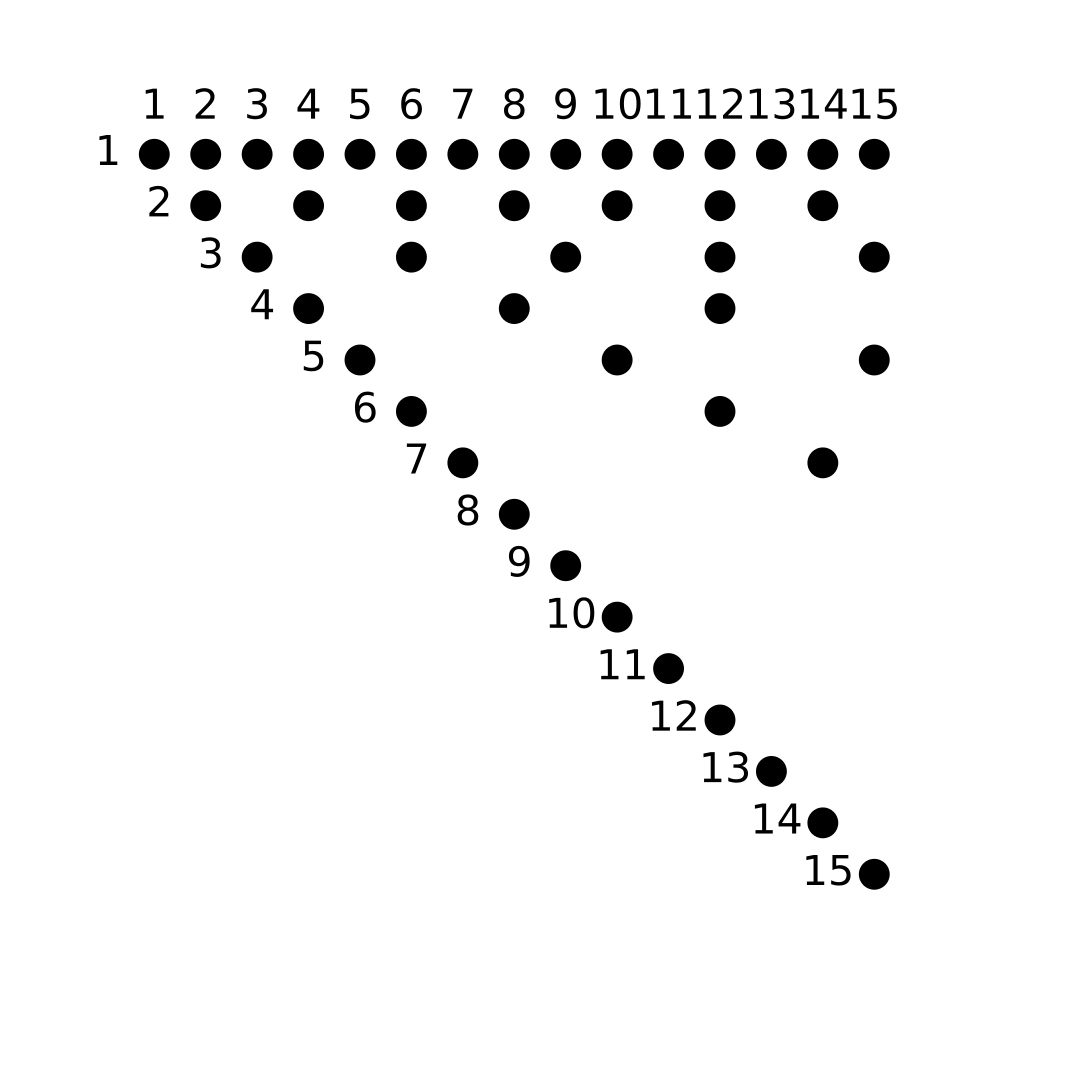
\includegraphics[height=0.85\textheight,keepaspectratio]{fotos/plain.png}
\end{frame}

\begin{frame}
  \centering
  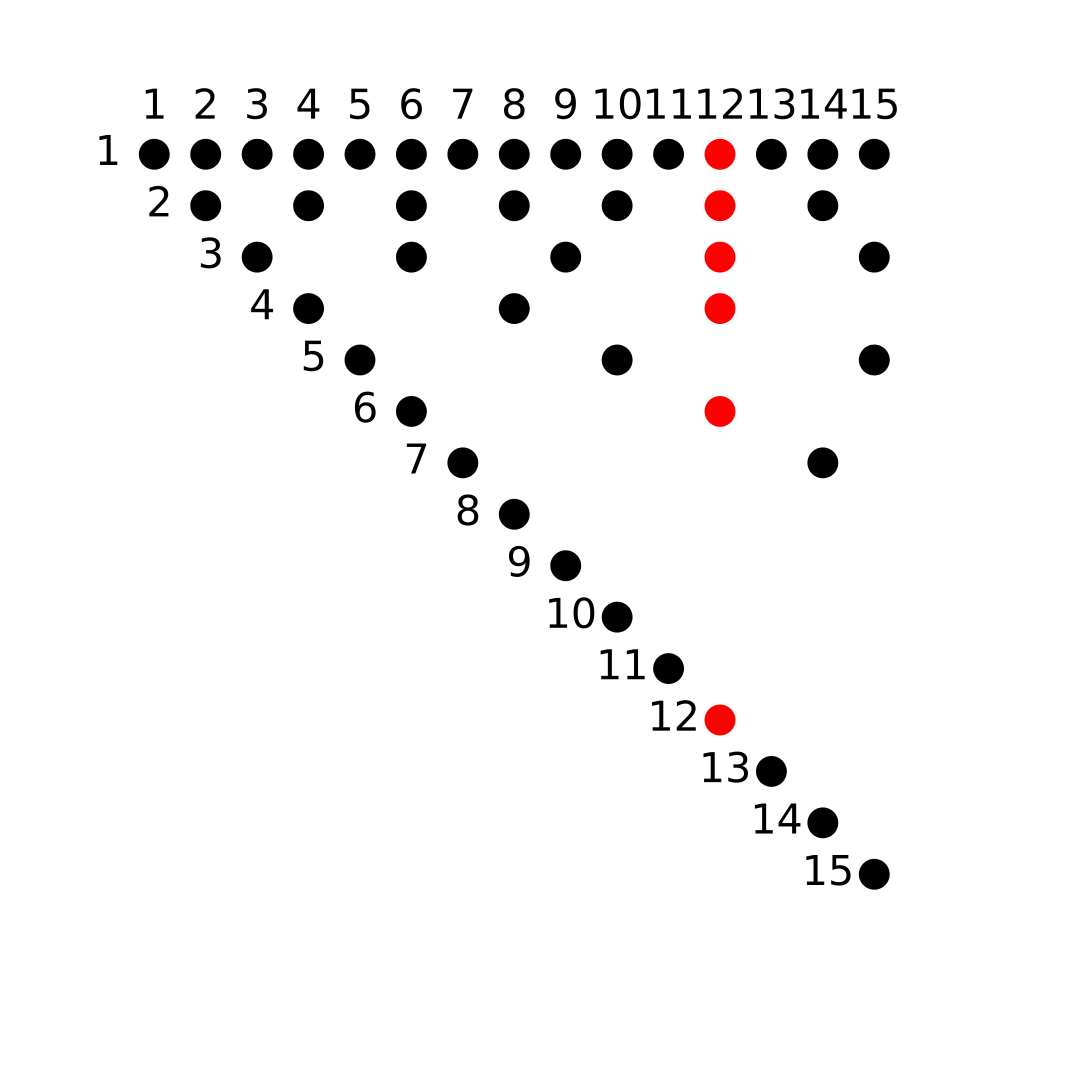
\includegraphics[height=0.85\textheight,keepaspectratio]{fotos/divisors.png}
\end{frame}

\begin{frame}
  \centering
  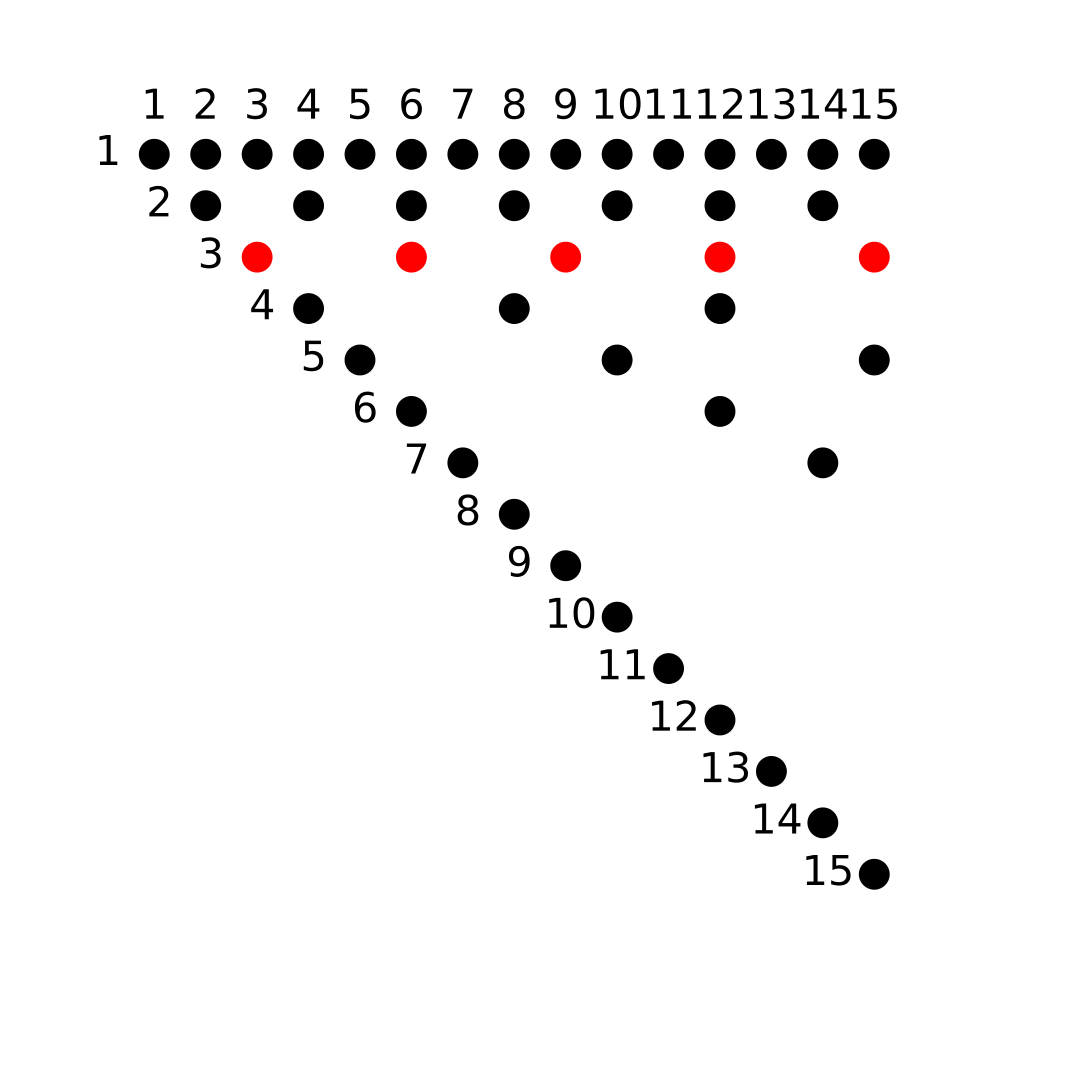
\includegraphics[height=0.85\textheight,keepaspectratio]{fotos/multiples.png}
\end{frame}

\begin{frame}
  \frametitle{Conteo doble}

  \[
    M_N(m) = \{ \text{múltiplos de } m \text{ menores o iguales a } N \}
  \]

  \[
    \frac{1}{N} \sum_{m=1}^{N} |M_N(m)|
    = \frac{1}{N} \sum_{m=1}^{N} \left\lfloor \frac{N}{m} \right\rfloor
    \leq \frac{1}{N} \sum_{m=1}^{N} \frac{N}{m}
    = \sum_{m=1}^{N} \frac{1}{m}
    \in O(\log N)
  \]
\end{frame}

\begin{frame}
  \centering
  \Huge Árboles?
\end{frame}

\section{Consultas de subárboles}

\subsection{Preorden}

\begin{frame}
  \frametitle{Consultas de subárboles}

  Supongamos un árbol donde cada nodo tiene un valor numérico. Queremos soportar dos operaciones:

  \begin{itemize}
    \item \texttt{suma(u)}: devuelve la suma de todos los valores del subárbol enraizado en \(u\).
    \item \texttt{cambiar(u, x)}: reemplaza el valor del nodo \(u\) por \(x\).
  \end{itemize}
\end{frame}


\begin{frame}
  \centering
  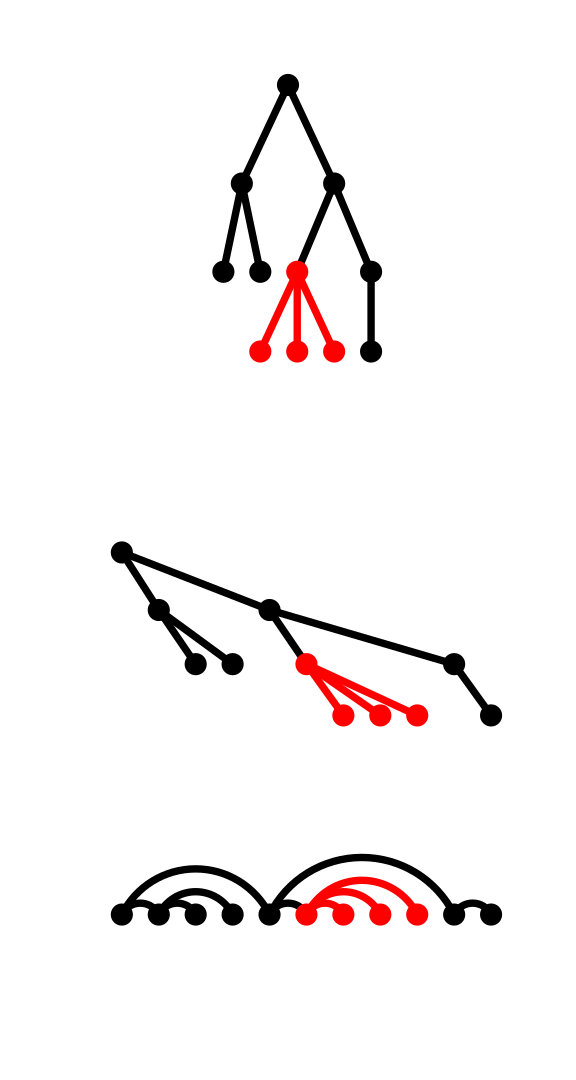
\includegraphics[height=1.05\textheight,keepaspectratio]{fotos/layouts.png}
\end{frame}


\begin{frame}
  \frametitle{Consultas de subárboles: idea}

  Podemos construir el \textbf{preorden} del árbol.

  \vspace{0.75em}

  \begin{itemize}
    \item Propiedad clave: a cada subárbol le corresponde un \textbf{subarray} en el preorden.
    \item Reducimos el problema a consultas en subarrays.
  \end{itemize}
\end{frame}


\begin{frame}[fragile]
  \frametitle{Consultas de subárboles: código}

\begin{lstlisting}
            int lp[maxn], rp[maxn];
            vector<int> pre;
            void dfs(int u, int p) {
                lp[u] = sz(pre);
                pre.push_back(val[u]);
                for (int v : g[u]) if (v != p) {
                    dfs(v, u);
                }
                rp[u] = sz(pre);
            }
            
            int suma(int u) {
                return suma_subarray(lp[u], rp[u]);
            }
\end{lstlisting}
\end{frame}

\begin{frame}
  \frametitle{Consultas de subárboles: observaciones}

  \begin{itemize}
    \item La misma solución sirve para máximos, mínimos, xor, gcd, etc.
    \item Sin embargo, \textbf{no funciona} para cualquier consulta que se nos ocurra.
    \item Por ejemplo: cantidad de números distintos, \texttt{mex} de los números, etc.
  \end{itemize}
\end{frame}

\section{Aristas livianas y pesadas}

\begin{frame}
  \centering
  \Huge Aristas livianas y pesadas
\end{frame}

\begin{frame}
  \frametitle{Ehad and the Big Finale (Codeforces 1174F)}

  \begin{itemize}
    \item Problema interactivo.
    \item Hay un árbol con raíz que tiene un nodo especial secreto \(\star\).
    \item \(N \le 10^5\).
    \item Te dan el árbol pero no te dicen cuál es el nodo secreto.
    \item Objetivo: descubrir el nodo secreto.
  \end{itemize}
\end{frame}

\begin{frame}
  \frametitle{Ehad and the Big Finale (Codeforces 1174F)}

  \begin{itemize}
    \item Para esto se pueden hacer dos tipos de consultas:
    \begin{itemize}
      \item \(d(u, \star)\): distancia de \(u\) al nodo especial.
      \item \(s(u)\): siguiente nodo en el camino de \(u\) a \(\star\).
    \end{itemize}
    \item Solo se pueden hacer 36 consultas.
    \item Solo se puede hacer la consulta \(s\) si \(u\) es ancestro de \(\star\).
    \item (Sin esta restricción se puede resolver haciendo consultas \(s\) en los centroides.)
  \end{itemize}
\end{frame}

\subsection{Definiciones}

\begin{frame}
  \frametitle{Aristas livianas y pesadas}

  Consideramos un árbol de \(N\) nodos.

  \vspace{0.75em}

  \begin{itemize}
    \item Por cada nodo con hijos, designamos como \textbf{hijo pesado} a aquel cuyo subárbol tiene la máxima cantidad de nodos (si hay más de uno, elegimos uno arbitrariamente).
    \item A las aristas que conectan nodos con su hijo pesado las llamamos \textbf{pesadas}.
    \item Si una arista no es pesada, la llamamos \textbf{liviana}.
    \item Terminología: a los caminos maximales formados enteramente por aristas pesadas los llamamos \textbf{caminos pesados}.
  \end{itemize}
\end{frame}

\begin{frame}
  \centering
  
\includegraphics[height=0.85\textheight,keepaspectratio]{fotos/heavy.png}
\end{frame}

\begin{frame}
  \frametitle{Aristas livianas y pesadas: observaciones}

  \begin{block}{Observación clave}
    En un camino nodo--raíz puede haber a lo sumo \(\log_2 N\) aristas livianas.
  \end{block}

  \begin{center}
    \fbox{\parbox{0.85\textwidth}{\centering\vspace{1.5cm}\textit{[Diagrama: camino a la raíz con $\le \log_2 N$ aristas livianas]}\vspace{1.5cm}}}
  \end{center}
\end{frame}

\begin{frame}
  \frametitle{Aristas livianas y pesadas: más observaciones}

  \begin{block}{Observación clave}
    Claim similar para cantidad de caminos pesados que se tocan.
  \end{block}

  \vspace{0.5em}

  Otra forma de verlo: dado un camino cualquiera, puede tocar a lo sumo \(2 \log_2 N\) aristas livianas. A su vez, cada vez que toca una arista liviana cambia de camino pesado, por lo que puede tocar a lo sumo \(2 \log_2 N + 1\) caminos pesados distintos.

  \vspace{0.5em}

  O sea, un camino cualquiera se puede descomponer en ``pocas'' partes, cada una perteneciente a un camino pesado distinto.
\end{frame}

\begin{frame}[fragile]
  \frametitle{Heavy-light decompose: código}

\begin{lstlisting}
int n;
vector<int> g[maxn];

int s[maxn]; // tamano del subarbol
int p[maxn]; // padre (-1 si no tiene)
int h[maxn]; // hijo pesado (-1 si no tiene)

// calculo padres y tamanos de los subarboles
void dfs(int u) {
    s[u] = 1;
    for (int v : g[u]) if (v != p[u]) {
        p[v] = u;
        dfs(v);
        s[u] += s[v];
    }
}

void decompose(int root) {
    p[root] = -1;
    dfs(root);

    forn(u, n) {
        h[u] = -1;
        for (int v : g[u]) if (v != p[u]) {
            if (h[v] == -1 || s[h[v]] < s[v]) {
                h[u] = v;
            }
        }
    }
}
\end{lstlisting}
\end{frame}


\begin{frame}
  \frametitle{Ehad and the Big Finale -- solución}

  Nos paramos en la raíz y vamos bajando hasta llegar a \(\star\), sin salirnos del camino de los ancestros de \(\star\) (para poder usar la consulta \texttt{s}).

  \vspace{0.75em}

  La idea del algoritmo es ir caminando de la raíz hasta \(\star\), pero saltando de un camino pesado al siguiente en cada paso: si estamos en un camino pesado, saltar rápido a la posición en la que el camino hacia \(\star\) se sale del camino pesado.
\end{frame}

\begin{frame}
  \frametitle{Consultas \texttt{d} en un camino pesado}

  Al estar en un camino pesado podemos hacer 2 consultas \texttt{d}(-):
  \begin{itemize}
    \item una en el nodo de arriba de todo (\(u\)),
    \item otra en el de abajo de todo (\(v\)).
  \end{itemize}

  \vspace{0.75em}

  Al saber las distancias \(u\text{-}\star\) y \(v\text{-}\star\), y la distancia \(u\text{-}v\), podemos calcular el punto en el que el camino raíz-\(\star\) se sale del camino pesado \(u\text{-}v\).
\end{frame}

\begin{frame}
  \frametitle{Localizar la salida con \texttt{d}(u) y \texttt{d}(v)}

  \centering
  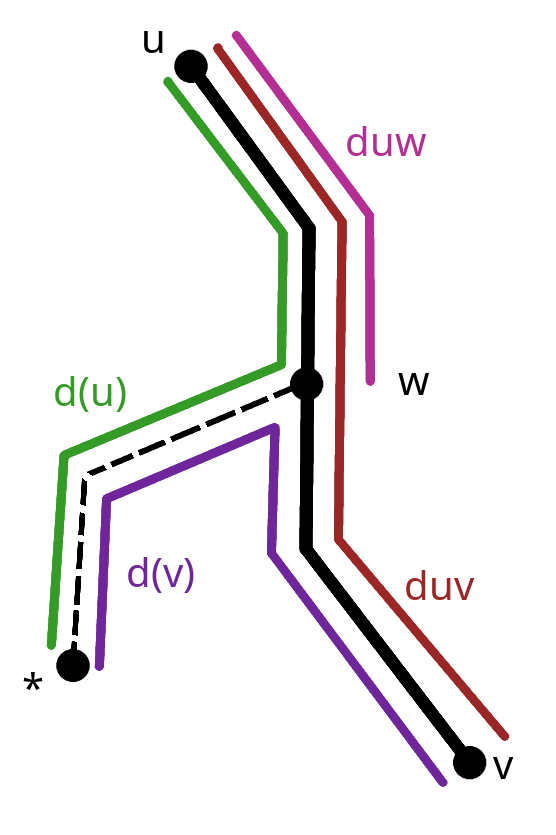
\includegraphics[height=0.55\textheight,keepaspectratio]{fotos/jumps.png}

  \vspace{0.4em}

  \[
    \text{duw} = \frac{duv + d(u) - d(v)}{2}
  \]

\end{frame}

\begin{frame}
  \frametitle{Cruzar la arista liviana}

  Una vez que sabemos el punto en el que se sale, sabemos que ahí hay que cruzar una arista liviana, pero no sabemos cuál.

  \vspace{0.75em}

  Para resolver eso hacemos una consulta \texttt{s}(-).

  \vspace{0.75em}

  Como nos mantenemos siempre en un camino nodo-raíz, la cantidad de aristas livianas y caminos pesados que tocamos es a lo sumo \(\log_2(N)\).

  \vspace{0.75em}

  Ahí tenemos una solución en \(3\log(N)\) consultas.
\end{frame}

\begin{frame}
  \frametitle{Optimización a \(2\log(N)+1\)}

  Se puede optimizar a \(2\log(N)+1\) evitando hacer consultas \texttt{d} en el nodo \(u\) en cada camino pesado: hacemos una consulta \texttt{d(raíz)} al principio y por cada paso que damos le restamos uno.
\end{frame}

\begin{frame}[fragile,shrink=5]
  \frametitle{Código: \texttt{special()}}

\begin{lstlisting}[basicstyle=\ttfamily\scriptsize]




                    int special() {
                        int u = 0;
                        int du = d(u);
                        while (true) {
                            if (du == 0) return u;
                            int duv = 0;
                            int v = u;
                            while (h[v] != -1) v = h[v], duv += 1;
                            int dv = d(v);
                            int steps = (du - dv + duv) / 2;
                            forn(_, steps) u = h[u], du -= 1;
                            if (du == 0) return u;
                            u = s(u);
                            du -= 1;
                        }
                    }
\end{lstlisting}
\end{frame}

\subsection{Consultas de subárbol exóticas}

\begin{frame}
  \frametitle{Distinct Colors (CSES 1139)}

  \begin{itemize}
    \item Hay un árbol enraizado en el nodo 1, con numeritos \(c_i\) en cada nodo \(i\).
    \item \(N \le 2 \cdot 10^5\).
    \item Por cada subárbol queremos saber la cantidad de valores distintos que contiene.
  \end{itemize}
\end{frame}

\begin{frame}
  \frametitle{Distinct Colors}

  \begin{itemize}
    \item Solucion Naive: Por cada nodo, metemos todos los valores del subárbol en un \texttt{set} y devolvemos \texttt{size()}.
    \item Costo: \(O(N^2)\).
    \item Para construir el conjunto de colores de un subarbol, podemos reutilizar el conjunto de colores de alguno de sus hijos. En particular, el del hijo pesado, ya que es el más grande.
    \item Esto seguro es más rápido, pero ¿cambia el costo asintótico? Resulta que sí, veamos por qué.
  \end{itemize}

\end{frame}

\begin{frame}[fragile]
\frametitle{Detalle del algoritmo}

En vez de pensarlo como una optimización, plantemos el algoritmo desde cero con esta idea de ir pasando el conjunto de colores de un hijo al padre.

Bajo esta perspectiva, contruimos un conjunto a medida que recorremos un camino pesado de abajo hacia arriba, agregando los colores de los descendientes faltantes de cada nodo. (los que no estan en el subarbol pesado)

\begin{lstlisting}[language={},basicstyle=\ttfamily\small]
    for p : caminos_pesados
      s = {}
      for u : ascendente(p)
        for v : hijo liviano de u
          for w : subarbol(v)
            agregar color(w) a s
        respuesta[u] = tamano de s
\end{lstlisting}

\end{frame}


\begin{frame}[fragile]
  \frametitle{Distinct Colors: doble conteo}

Más allá del orden de iteración, nuestro algoritmo recorre los mismos valores que este otro:

\begin{lstlisting}[language={},basicstyle=\ttfamily\small]
    for u = 1..n
      for v : g[u]
        if u-v es liviana
          for w : subarbol(v)
            print(w, v, u)
\end{lstlisting}

O sea, itera por los pares \(\{(u, w) \mid u \in V,\ w \in D(u)\}\), donde

\centerline{$\displaystyle
  D(u) = \{ \text{descendientes de } u \text{ que no están en el subárbol pesado} \}
$}

\smallskip

Pero este es el mismo conjunto de pares que \(\{(u, w) \mid w \in V,\ u \in A(w)\}\), donde

\centerline{$\displaystyle
  A(w) = \{ \text{ancestros de } w \text{ con arista liviana hacia } w \}
$}

El cual es claramente \(O(N \log N)\), porque por cada \(w\) hay solo \(\log_2(N)\) aristas livianas en su camino a la raíz.

\end{frame}

\begin{frame}[fragile]
  \frametitle{Distinct Colors: código}

\begin{lstlisting}
    vector<int> distintos() {
        vector<int> ans(n);
        unordered_set<int> s;
        forn(f, n) if (h[f] == -1) {
            int u = f;
            while (true) {
                s.insert(u);
                for (int v : g[u]) if (v != p[u] && v != h[u])
                    meter_todo(v, u, s);
                ans[u] = s.size();
                int w = p[u];
                // corto al llegar al tope del camino pesado
                if (w == -1 || h[w] != u) break;
                u = w;
            }
            s.clear();
        }
        return ans;
    }
\end{lstlisting}
\end{frame}


\subsection{LCA}

\begin{frame}
  \frametitle{Mandatory LCA slide (again)}

  \centering
  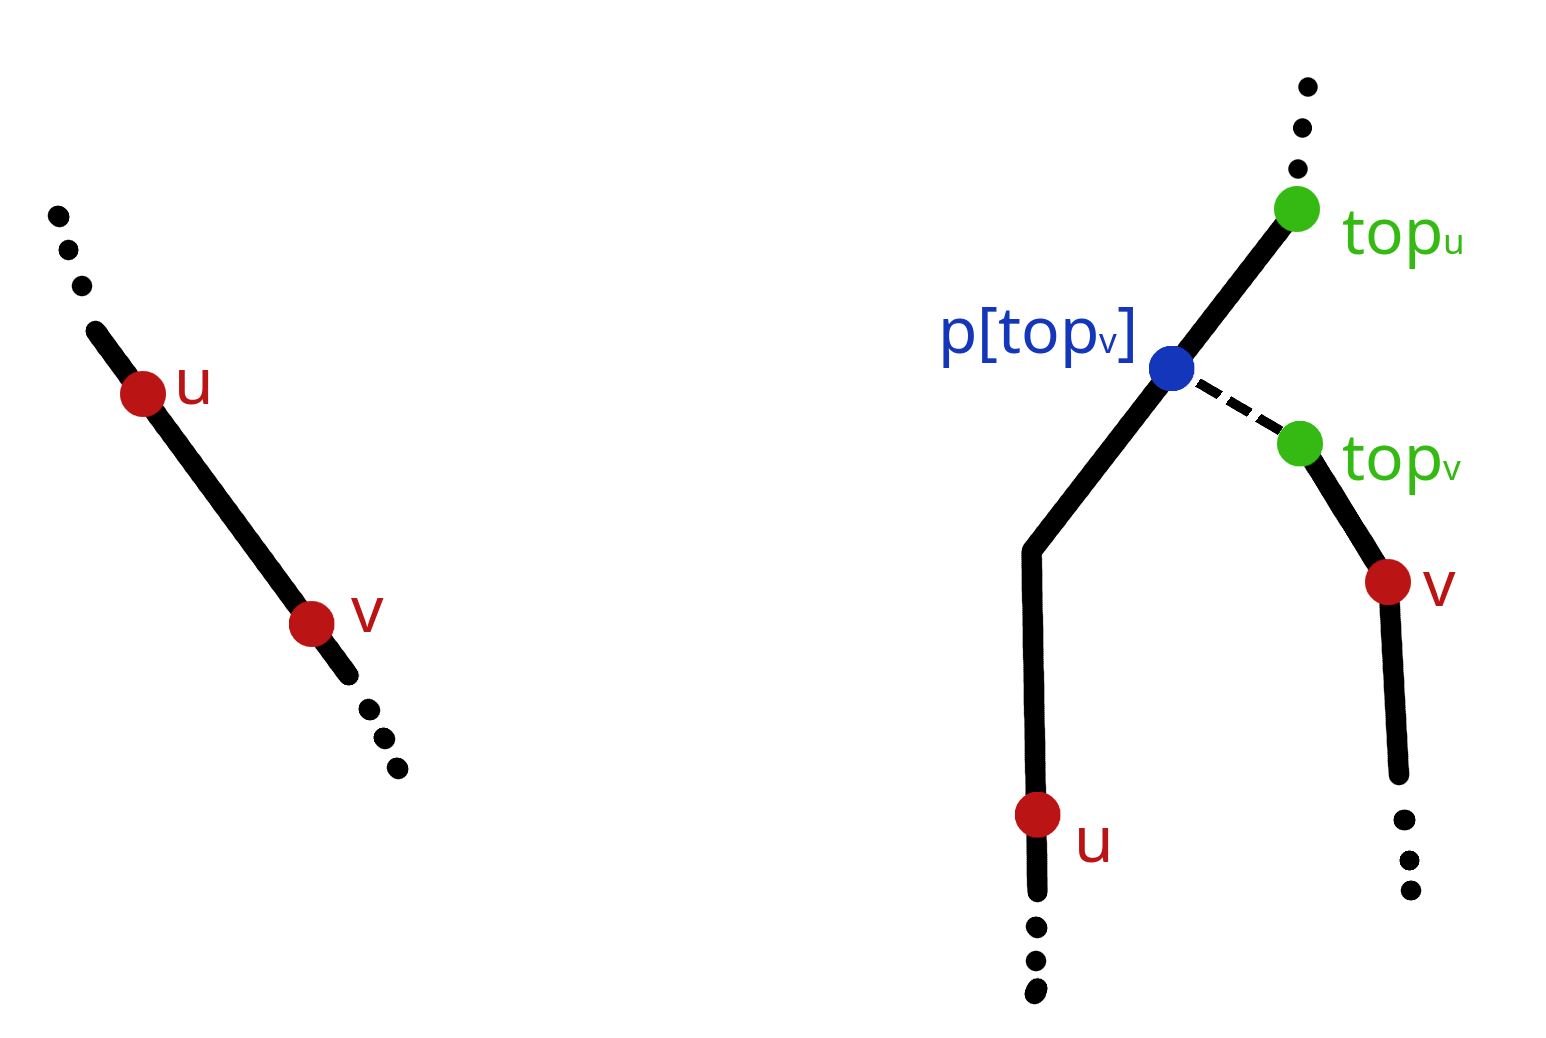
\includegraphics[height=0.85\textheight,keepaspectratio]{fotos/lca.png}
\end{frame}

\begin{frame}[fragile]
  \frametitle{Mandatory LCA slide (again)}
  \begin{lstlisting}
int lca(int u, int v) {
    int tu = htop[u], tv = htop[v];
    if (tu == tv) {
        if (dep[u] > dep[v]) swap(u, v);
        return u;
    } else {
        if (dep[tu] < dep[tv]) swap(u, v), swap(tu, tv);
        return lca(p[tu], v)
    }
}
  \end{lstlisting}
\end{frame}
\section{Consultas de caminos}

\subsection{Problema}

\begin{frame}
  \centering
  \huge Consultas de caminos
\end{frame}

\begin{frame}
  \frametitle{Consultas de caminos usando la descomposición}

  Tenemos un árbol con números en los nodos. Queremos soportar dos operaciones:

  \begin{itemize}
    \item \texttt{suma(u, v)}: devuelve la suma de todos los números del camino \(u\)--\(v\)
    \item \texttt{cambiar(u, x)}: reemplaza el número del nodo \(u\) con \(x\)
    \item \(N \le 2 \cdot 10^5\)
    \item \(Q \le 2 \cdot 10^5\)
  \end{itemize}
\end{frame}

\subsection{Descomposición en caminos pesados}

\begin{frame}
  \frametitle{Consultas de caminos: descomposición}

  La idea es nuevamente aprovechar que cualquier camino se puede descomponer en varios pedazos, cada uno parte de un camino pesado distinto, y que esta descomposición tiene pocas partes (\(O(\log N)\)).
\end{frame}

\begin{frame}
  \frametitle{Consultas de caminos: descomposición}

  \begin{center}
    
\includegraphics[height=0.85\textheight,keepaspectratio]{fotos/heavy-paths.png}
  \end{center}
\end{frame}

\begin{frame}
  \frametitle{Consultas de caminos: consultas por pedazo}

  Para resolver la suma dentro de cada pedazo necesitamos poder hacer consultas de rango en el array de elementos del camino pesado.

  \vspace{0.75em}

  La forma clásica es construir un \textbf{segment tree} sobre cada camino pesado.
\end{frame}



\begin{frame}
  \frametitle{Consultas de caminos: idea del algoritmo}

  \begin{itemize}
    \item Si el camino está completamente contenido en un camino pesado, hacemos la consulta directamente.
    \item Si no, el camino \(u\)--\(v\) necesariamente llega hasta la cima de un camino pesado y se sale hacia arriba.
    \item Detectamos cuál de las dos puntas es la que se sale por la cima, y hacemos la consulta en ese camino pesado.
    \item De esta forma resolvemos la punta del camino \(u\)--\(v\) y achicamos el camino que falta por resolver.
  \end{itemize}

  \vspace{0.75em}

\end{frame}

\begin{frame}[fragile]
  \frametitle{Consultas de caminos: consulta}

\begin{lstlisting}
int query(int u, int v) {
  int tu = htop[u], tv = htop[v];
  if (tu == tv) {
    if (dep[u] > dep[v]) swap(u, v);
    return tree[tu].query(dep[u]-dep[tu], dep[v]-dep[tu]+1);
  } else {
    if (dep[tu] < dep[tv]) swap(u, v), swap(tu, tv);
    return tree[tu].query(0, dep[u]-dep[tu]+1) + query(p[tu], v);
  }
}
\end{lstlisting}
\end{frame}
\subsection{Operaciones no conmutativas}

\begin{frame}
  \frametitle{Consultas no conmutativas}

  El algoritmo de consultas en caminos funciona también para operaciones \textbf{no conmutativas} (por ejemplo, producto de matrices).

  \vspace{0.75em}

  \begin{itemize}
    \item Guardamos pares con la suma de izquierda a derecha y la suma de derecha a izquierda.
    \item En cada paso del algoritmo elegimos la dirección correcta según cuál punta del camino estamos resolviendo.
  \end{itemize}
\end{frame}

\begin{frame}[fragile]
  \frametitle{Consultas no conmutativas: estructuras}

\begin{lstlisting}
struct Mono {
    static Mono neut() { /* ... */ }
};
Mono operator + (Mono x, Mono y);

struct Conm {
    Mono ltr, rtl;
    static Conm make(Mono x) { return {x, x}; }
    static Conm neut() { return {Mono::neut(), Mono::neut()}; }
};
Conm operator + (Conm x, Conm y) {
    return {x.ltr + y.ltr, y.rtl + x.rtl};
}
\end{lstlisting}
\end{frame}

\begin{frame}[fragile]
  \frametitle{Consultas no conmutativas: \texttt{query}}

\begin{lstlisting}
Mono query(int u, int v) {
  int tu = htop[u], tv = htop[v];
  if (tu == tv) {
    if (dep[u] < dep[v]) {
      return tree[tu].query(dep[u]-dep[tu],dep[v]-dep[tu]+1).ltr;
    } else {
      return tree[tv].query(dep[v]-dep[tv],dep[u]-dep[tv]+1).rtl;
    }
  } else {
    if (dep[tu] > dep[tv]) {
      return tree[tu].query(0, dep[u]-dep[tu]+1).rtl
           + query(p[tu], v);
    } else {
      return query(u, p[tv])
           + tree[tv].query(0, dep[v]-dep[tv]+1).ltr;
    }
  }
}
\end{lstlisting}
\end{frame}

\section{Euler tour}

\begin{frame}
\centering
\huge Euler Tour
\end{frame}

\begin{frame}
  \frametitle{Consultas de xor en caminos (sin updates)}

  \begin{itemize}
    \item Te dan un arbol con numeros en las aristas
    \item Querés soportar consultas de xor en caminos
    \item \(N \leq 2 \cdot 10^5\)
    \item \(Q \leq 2 \cdot 10^5\)
  \end{itemize}
  Esto se puede resolver descomponiendo en caminos pesados.

  \vspace{0.75em}

  Pero también hay una solución muchísimo más simple.
\end{frame}

\begin{frame}
  \frametitle{Consultas de xor en caminos: idea}

  La idea es construir el \textbf{Euler tour}: un array de los valores de aristas en el orden en que te los encontrás si hacés un DFS del árbol.

  \vspace{0.75em}

  \begin{itemize}
    \item Se inserta el valor tanto al \textbf{ir} como al \textbf{volver} de cada arista.
    \item Para responder una consulta de xor en un camino \(u\)--\(v\), consultamos en ese array. El rango corresponde a las posiciones de \(u\) y \(v\) en el recorrido.
  \end{itemize}
\end{frame}

\begin{frame}
  \frametitle{Consultas de xor en caminos: por qué funciona}

  Si mirás el intervalo de valores entre una aparición de \(u\) y una de \(v\), cualquier arista por la que ``fuimos y volvimos'' entre medio en el DFS se cancela, porque el xor es su propia inversa.

  \vspace{0.75em}

  Y coincidentemente esas aristas son las que \textbf{no} están en el camino \(u\)--\(v\). O sea, las que no se cancelan son exactamente las del camino \(u\)--\(v\).

  \vspace{0.75em}

  Por lo tanto, la respuesta es simplemente el xor de los valores de las aristas en el camino \(u\)--\(v\).
\end{frame}

\begin{frame}[fragile]
  \frametitle{Consultas de xor en caminos: código}

\begin{lstlisting}
struct edge {
    int u, v, x;
    int opp(int w) { return u + v - w; }
}
edge edges[maxn];
vector<int> g[maxn];
vector<int> euler_tour;
int position[maxn];
void dfs(int u, int p) {
    for (int i : g[u]) {
        edge e = edges[i];
        int v = e.opp(u);
        if (v == p) continue;

        position[u] = sz(euler_tour);
        euler_tour.push_back(e.x);
        position[v] = sz(euler_tour);
        dfs(v, u);
        euler_tour.push_back(e.x);
    }
}

void init() {
    dfs(0, -1);
    init_array(euler_tour);
}

void query(int u, int v) {
    int pu = position[u], pv = position[v];
    return xor_array(pu, pv);
}
\end{lstlisting}
\end{frame}

\subsection{Algoritmo de Mo}

\begin{frame}
  \frametitle{Consultas de caminos usando el truco de Mo}

  Esta idea es muy buena pero depende de propiedades particulares de la operación \texttt{xor}:

  \vspace{0.5em}

  \begin{itemize}
    \item es asociativa
    \item tiene elemento neutro
    \item tiene inverso para cada elemento
    \item es conmutativa
    \item \textbf{cada elemento es su propio inverso}
  \end{itemize}
\end{frame}

\begin{frame}
  \frametitle{Consultas de caminos usando el truco de Mo: generalización}

  En realidad se puede generalizar a cualquier operación si cumple las primeras 4.

  \vspace{0.75em}

  \begin{alertblock}{Nota}
    conmutativa es opcional pero complica la implementación
  \end{alertblock}
\end{frame}

\begin{frame}
  \frametitle{Consultas de caminos usando el truco de Mo: idea}

  Básicamente la idea es hacer un \texttt{for} desde la posición de \(u\) hasta la de \(v\), e ir acumulando los valores.

  \vspace{0.75em}

  A medida que hacemos esto, hay que chequear si estamos yendo o volviendo por una arista. En caso de estar yendo, acumulamos el valor de la arista. En caso de estar volviendo, acumulamos el inverso del valor de la arista.

  \vspace{0.75em}

  De esta forma, tenemos un algoritmo que funciona para una operación donde no necesariamente cada elemento es su propio inverso.
\end{frame}

\begin{frame}
  \frametitle{Consultas de caminos usando el truco de Mo: implementación}

  Para chequear esto, simplemente guardamos los índices de las aristas en el Euler tour en vez de los valores.

  \vspace{0.75em}

  Aparte, podemos mantener un array de booleanos que nos diga si ya sumamos el valor de la arista o no.
\end{frame}

\begin{frame}[fragile]
  \frametitle{Consultas de caminos usando el truco de Mo: código}

\begin{lstlisting}
bool tengo[maxn];
int query(int u, int v) {
    int ans = 0;
    int l = position[u], r = position[v];
    if (l > r) swap(l, r);
    for (int i = l; i < r; i++) {
        int j = euler_tour[i];
        if (tengo[j]) ans -= edges[j].x;
        else          ans += edges[j].x;
        tengo[j] = !tengo[j];
    }
    return ans;
}
\end{lstlisting}
\end{frame}

\begin{frame}
  \frametitle{Consultas de caminos usando el truco de Mo: complejidad}

  Esto funciona pero es horrendamente lento. Claramente hace un \texttt{for} \(O(N)\) por consulta.
\end{frame}

\subsection{Ordenamiento de Mo}

\begin{frame}[fragile]
  \frametitle{El truco de Mo}

  Fijate que realmente podemos extender y achicar el rango de la consulta:

\begin{lstlisting}
void metesaca(int j) {
    if (tengo[j]) {
        <saca>
    } else {
        <mete>
    }
    tengo[j] = !tengo[j];
}
\end{lstlisting}

  O sea, si tenemos en algún momento acumulado el intervalo \([l, r)\), podemos \emph{metesacar} (\(l-1\), \(l\), \(r-1\) o \(r\)) para obtener los intervalos \([l-1, r)\), \([l+1, r)\), \([l, r-1)\) o \([l, r+1)\).
\end{frame}

\begin{frame}
  \frametitle{El truco de Mo: movimiento en el plano}

  Si pensamos en el intervalo \([l, r)\) como un punto \((l,r)\) en el plano, podemos movernos hacia arriba, abajo, izquierda o derecha.

  \vspace{0.75em}

  A medida que nos movemos por el plano, podemos llegar a posiciones que se corresponden con las consultas que tenemos que hacer.

  En esos puntos, podemos guardar el valor acumulado para obtener la respuesta de la consulta.

  \vspace{0.75em}

  Resulta posible elegir un orden de movimiento tal que el costo total sea \(O((N + Q)\sqrt{N})\).
\end{frame}

\begin{frame}
  \centering
  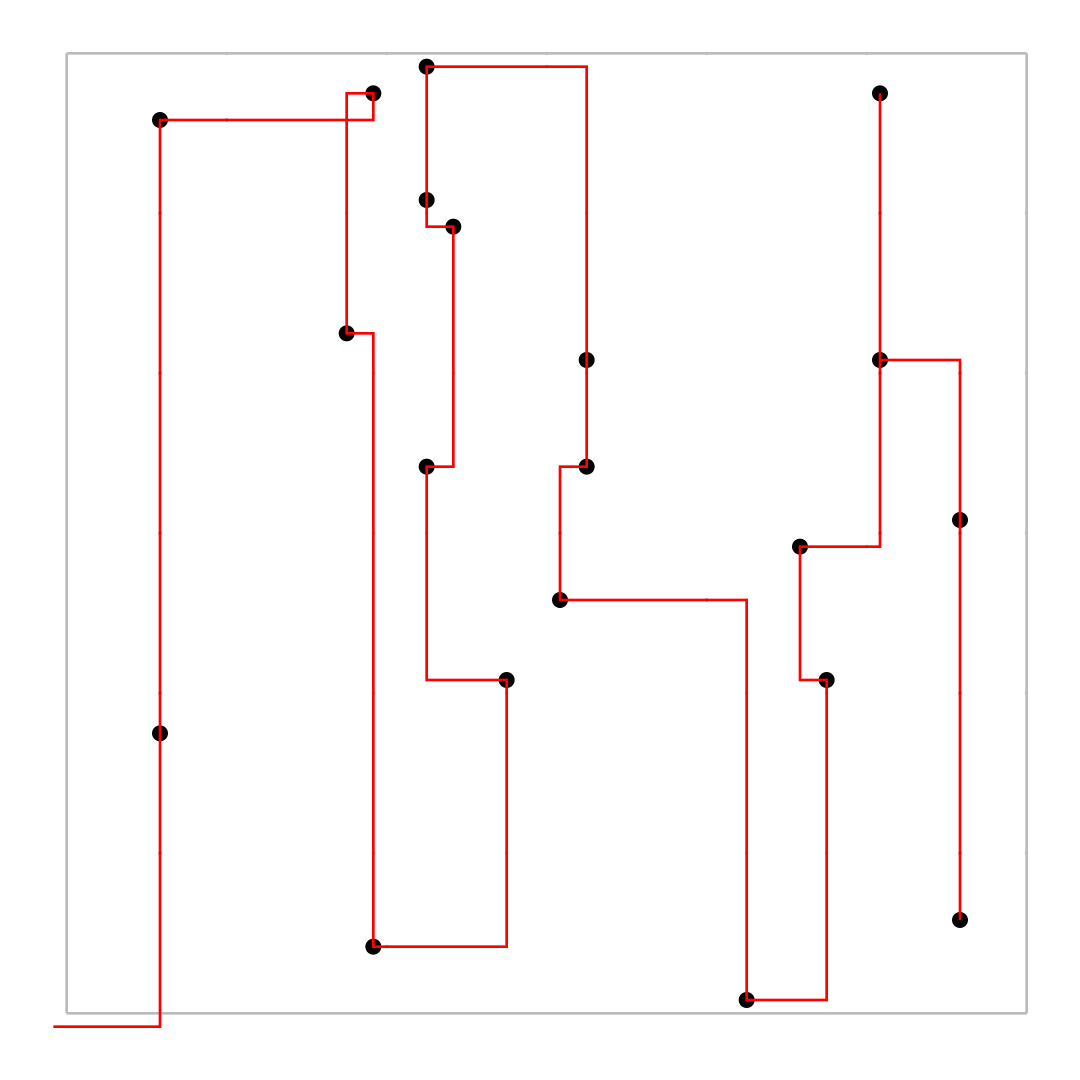
\includegraphics[height=0.85\textheight,keepaspectratio]{fotos/path-clean.png}
\end{frame}

\begin{frame}
  \frametitle{El truco de Mo: complejidad}

  Partimos el plano en cuadrados de \(\sqrt{N} \times \sqrt{N}\) y recorremos los cuadrados en zig zag.

  \vspace{0.75em}

  Pasar de cada punto al siguiente cuesta \(O(\sqrt{N})\) si está en el mismo bloque. En total sobre todos los puntos es \(O(Q\sqrt{N})\).

  \vspace{0.75em}

  Podemos considerar por separado el caso de cambiar de bloque.

  En total hay \(O(N)\) bloques, y moverse de uno a otro cuesta \(O(\sqrt{N})\). En total es \(O(N\sqrt{N})\).

  \vspace{0.75em}

  Entonces, el costo total es \(O((Q + N)\sqrt{N})\).
\end{frame}

\begin{frame}
  \centering
  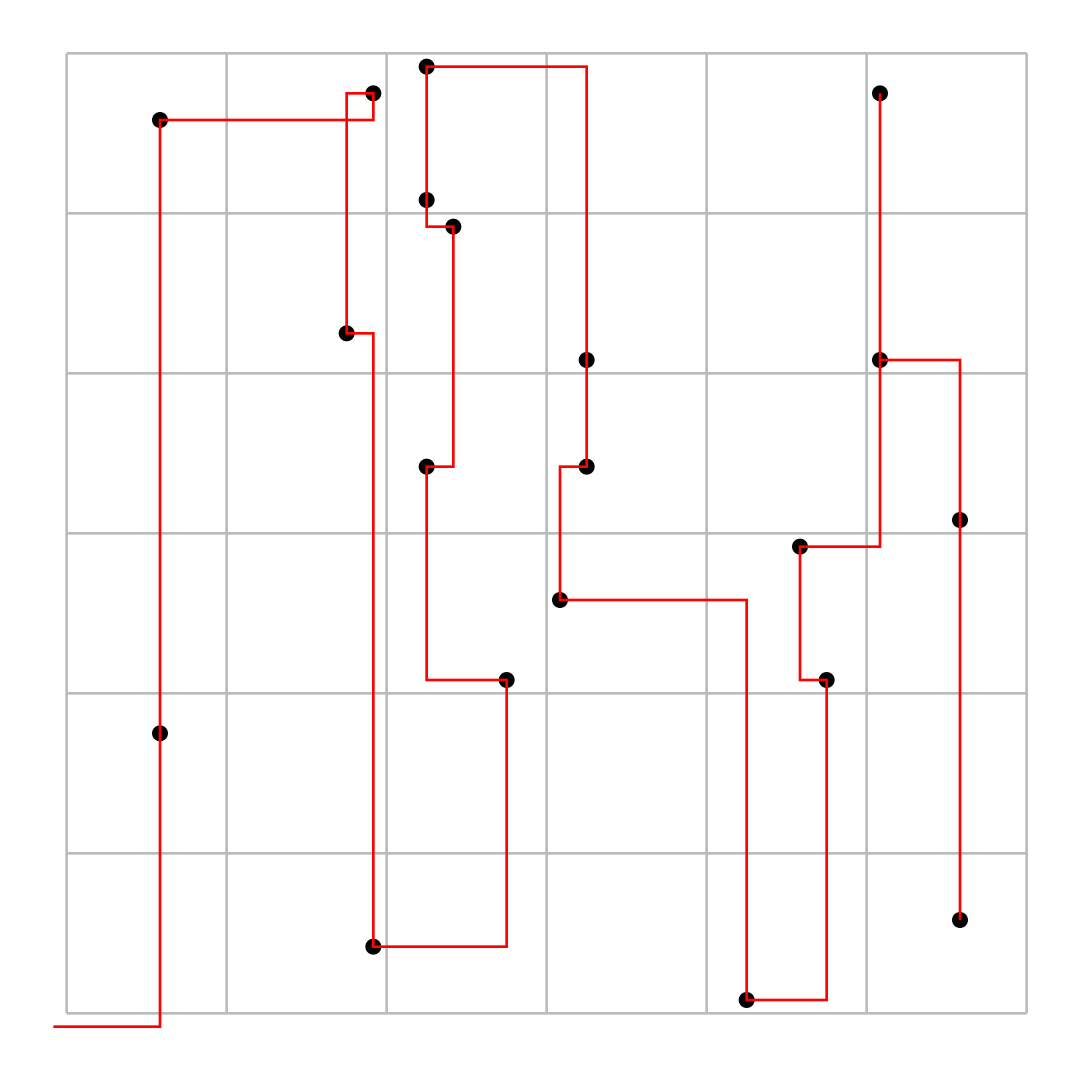
\includegraphics[height=0.85\textheight,keepaspectratio]{fotos/path.png}
\end{frame}

\begin{frame}[fragile]


  \begin{lstlisting}

              vector<int> perm = orden_mo(queries);
              int l = 0, r = 0;
              for (int i : perm) {
                  auto [ql, qr] = queries[i];
                  while (ql < l) metesaca(--l);
                  while (r < qr) metesaca(r++);
                  while (l < ql) metesaca(l++);
                  while (qr < r) metesaca(--r);
                  ans[i] = <respuesta>
              }
  \end{lstlisting}
\end{frame}

\begin{frame}
  \centering
  \huge Gracias
\end{frame}

\end{document}
